\chapter{环境}

\section{为什么要自己排版?}
\label{sec:whyTypesetting}

如果是纯文学著作,完全可以交给出版社去排版。
但是对于编程技术书籍,文字之间还穿插代码和图表,
那么出版社的专业排版人员很难排出符合程序员审美观的版面,
甚至有可能造成技术错误。


\begindot
\item 代码的排版,注意分页和折行。特别是Python这种缩进敏感的语言,
一般要避免在一个函数内分页,这会造成阅读困难。可以在函数定义之间分页。

\item 写作与排版一体化,作者可以适当改写内容,让版面更美观。
例如,假如一个函数最后一行那个花括号被挤到了下一页第一行,这就很难看。
这时可以考虑临时改变代码的缩进(从BSD风格改为K\&R风格),从而节省一两行空间,
让花括号落在本页。另外也可以稍微改变说法,避免段尾孤字成行。
\myenddot


\section{为什么要用\LaTeX排版?}
\begindot
\item \LaTeX 可以处理英文断字(Hyphenation),避免一行文字太稀疏。
例如\fn{Concurrent\-Hash\-Map} 这种在技术书籍中经常出现的长类名,
如果不断字就会造成难看的版面。这也是Word排版容易出现的问题。
另外\LaTeX的断行和断页采用动态规划算法,排出来的版面比Word的贪心算法更匀称。

\item \LaTeX 的源文件是文本格式,可以方便地做版本管理(\fn{diff}/\fn{merge}),
并且很容易利用和编写各种小工具来处理它。
相反Word的 \fn{.doc}/\fn{.docx} 文件处理起来就麻烦多了,如果不是不可能的话
(想想一句 \fn{grep | sort | uniq -c} 要写多少代码)。

\item \LaTeX 可以方便地做出交叉引用,引用其他章节图表的页码或编号。
\LaTeX 原稿可以分散到多个 \fn{.tex} 文件中,便于编辑。
如果 Word 也这么做(每章一个文件),那么交叉引用就麻烦得多。
但是如果把整本书做成一个Word文件,那编辑起来就困难多了,牵一发而动全身。
而且有一种如履薄冰的感觉,生怕哪天文件突然就损坏了。
\myenddot

\subsection{动手之前}
作者有能力并且有意愿完整书籍的排版,向出版社提供印刷质量的PDF文稿。
出版社愿意改变通常的工作流程,采用作者提供的PDF文件来校对并印刷。
\LaTeX 不是一个傻瓜化的工具,它需要投入相当的精力去学习,才能排出满意的效果。

%\section{硬件设备}
%我自己使用两台24吋显示器,并排

\section{软件工具}
%本节介绍我的排版工作环境。

\subsection{\TeX 发行版}
Linux用TeX Live,Windows用CTeX套装,Mac OS X 用 Mac TeX。
中文处理采用xelatex + xeCJK + ctex 方案
\footnote{\myurl{http://blog.jjgod.org/2009/11/21/chinese-in-tex-live-2009/}},
不要采用过时的 CJK 或 CCT 方案。

注意,\TeX本身是非常稳定的,但是中文处理则在不断改进。
例如TeX Live 2010和TeX Live 2012在处理中英文混排方面就有区别,
造成“动版”,严重时会影响既有分页。

\vspace{1ex}
\centerline{\fbox{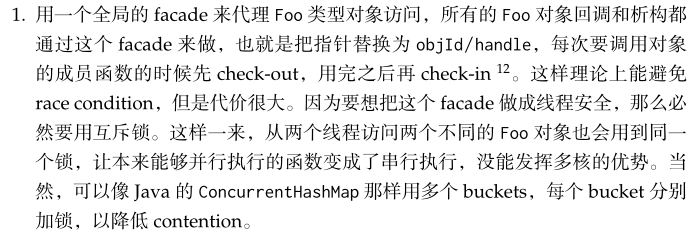
\includegraphics[width=360pt]{texlive2010.png}}}

\vspace{1ex}
\centerline{\fbox{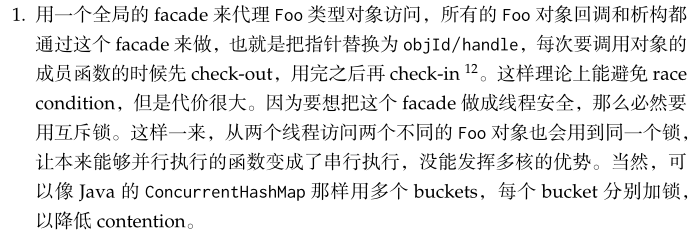
\includegraphics[width=360pt]{texlive2012.png}}}

\vspace{1ex}
因此我建议不要在排版期间升级 \LaTeX 的版本,
这也是我在虚拟机上安装 TeX Live 的原因之一。

\subsection{操作系统}
有好用的中文输入法,能方便地用命令行处理文本文件(\fn{grep}、\fn{sort}、\fn{awk} 等)。

因此我用的是一种混合办法,笔记本上安装Windows,
再在虚拟机中安装Debian Linux,
然后在Debian 中安装 TeX Live。
最后用Samba共享文件夹,这样就可以在Windows下方便地编辑Linux上的文件。
而在Linux上用 Git 管理 \fn{.tex} 源文件和图片。

%\subsection{文本编辑器}
%任何
\subsection{PDF阅读器}
推荐SumatraPDF,它不锁PDF文件,可以随时覆盖,并且自动刷新。
\subsection{绘图工具}

\section{文档结构}
\subsection{UTF-8编码}
\subsection{\fn{.tex} 文件组织}
文件名
不要有下划线

\section{版本管理}
\subsection{理想的工作流程}
\subsection{现实的工作流程}

